\documentclass[margin=0mm,tikz]{standalone}

\usepackage{tikz}
\usepackage{xcolor}
\usepackage{ifthen}
%\usepackage{mathtools}
%\usepackage{stackengine}

\usetikzlibrary{positioning}
\usetikzlibrary{fit}
\usetikzlibrary{calc}
\usetikzlibrary{arrows.meta}
\usetikzlibrary{quotes}

\pgfdeclarelayer{background}
\pgfsetlayers{background,main}

% -----------------------
% colors
% -----------------------
\definecolor{convcolor}{RGB}{175, 0, 23}
\definecolor{convblockcolor}{RGB}{0, 93, 157}
\definecolor{downscalecolor}{RGB}{48, 11, 213}
\definecolor{upscalecolor}{RGB}{11, 176, 213}
\definecolor{forwardcolor}{RGB}{100, 100, 100}
\definecolor{skipcolor}{RGB}{218, 138, 0}
\definecolor{operatorcolor}{RGB}{136, 150, 186}
\definecolor{reccolor}{RGB}{113, 0, 162}
\definecolor{catcolor}{RGB}{255, 0, 0}


% Set background color
%\pagecolor{white}

% -----------------------
% styles
% -----------------------

\tikzstyle{operator} = [
    circle,
    draw,
    top color = gray!20!white,
	bottom color = gray!30!white,
    text=black,
    minimum size=0.5cm,
    inner sep=0pt
]

\tikzstyle{conv} = [-{Latex[length=6pt, width=10pt]}, line width=3pt, convcolor]
\tikzstyle{convblock} = [-{Latex[length=6pt, width=10pt]}, line width=3pt, convblockcolor]
\tikzstyle{downscale} = [-{Latex[length=6pt, width=10pt]}, line width=3pt, downscalecolor]
\tikzstyle{upscale} = [-{Latex[length=6pt, width=10pt]}, line width=3pt, upscalecolor]
\tikzstyle{forward} = [-{Latex[length=2pt, width=4pt]}, line width=1pt, forwardcolor]
\tikzstyle{skip} = [-{Latex[length=3pt, width=5pt]}, line width=2pt, skipcolor]
\tikzstyle{rec} = [-{Latex[length=6pt, width=10pt]}, line width=3pt, reccolor]
\tikzstyle{cat} = [dashed, line width=1pt, catcolor]


\tikzset{
	annotated cuboid/.pic={
		\tikzset{%
			every edge quotes/.append style={midway, auto},
			/cuboid/.cd,
			#1
		}

		% coordinate scheme of the cube
		%
		%    e---------h
		%   /|        /|
		%  / |       / |
		% a---------d  |
		% |  |      |  |
		% |  f------|--g
		% | /       | /
		% |/        |/
		% b---------c
		
		% Set up the corner coordinates of the cube
		\coordinate (a) at (-\cwidth*\cscale*0.5, \cheight*\cscale*0.5, 0);
		\coordinate (b) at (-\cwidth*\cscale*0.5, -\cheight*\cscale*0.5, 0);
		\coordinate (c) at (\cwidth*\cscale*0.5, -\cheight*\cscale*0.5, 0);
		\coordinate (d) at (\cwidth*\cscale*0.5, \cheight*\cscale*0.5, 0);
		\coordinate (e) at (-\cwidth*\cscale*0.5, \cheight*\cscale*0.5, -\cdepth*\cscale);
		\coordinate (f) at (-\cwidth*\cscale*0.5, -\cheight*\cscale*0.5, -\cdepth*\cscale);
		\coordinate (g) at (\cwidth*\cscale*0.5, -\cheight*\cscale*0.5, -\cdepth*\cscale);
		\coordinate (h) at (\cwidth*\cscale*0.5, \cheight*\cscale*0.5, -\cdepth*\cscale);
		

		% Clip the cube image to the outer coordinates
		\clip (a) -- (b) -- (c) -- (g) -- (h) -- (e) -- cycle;
		
		%
		% Draw the cube
		
		\draw[\ccolor, dashed, very thick] (f) -- (g);
		\ifthenelse{\cat=0}{
			\draw[\ccolor, dashed, very thick] (f) -- (b);
			\draw[\ccolor, dashed, very thick] (f) -- (e);
		}{
			\draw[catcolor, dashed, very thick] (f) -- (b);
			\draw[catcolor, dashed, very thick] (f) -- (e);
		}
		% Dashed, hidden lines
		%\draw[\ccolor, dashed, very thick] (f) -- (b);
		%\draw[\ccolor, dashed, very thick] (f) -- (g);
		%\draw[\ccolor, dashed, very thick] (f) -- (e);
		
		% Faces
		\draw[fill=\ccolor, opacity=0.6] (a) -- (b) -- (c) -- (d) -- cycle;  % front
		\draw[fill=\ccolor, opacity=0.6] (a) -- (d) -- (h) -- (e) -- cycle;  % top
		\draw[fill=\ccolor, opacity=0.6] (d) -- (c) -- (g) -- (h) -- cycle;  % right
		
		% Redraw edges of the faces
		\draw[\ccolor, very thick] (a) -- (b) -- (c) -- (d) -- cycle;  % front
		\draw[\ccolor, very thick] (a) -- (d) -- (h) -- (e) -- cycle;  % top
		\draw[\ccolor, very thick] (d) -- (c) -- (g) -- (h) -- cycle;  % right
		
		\ifthenelse{\cat=1}{
			\draw[catcolor, dashed, very thick] (b) -- (a) -- (e);
		}{}
		
		% Draw annotations
		\draw [\ccolor] (a) edge ["\color{black}\textbf{\lheight}"] (b);
		\draw [\ccolor] (b) edge ["\color{black}\textbf{\lwidth}"] (c);
	
		% Define the node for this kernel
		\node [anchor=north west, minimum width=\cwidth*\cscale cm, minimum height=\cheight*\cscale cm] (\clabel) at (a) {};
	
	},
	/cuboid/.search also={/tikz},
	/cuboid/.cd,
	width/.store in=\cwidth,
	height/.store in=\cheight,
	depth/.store in=\cdepth,
	units/.store in=\cunits,
	scale/.store in=\cscale,
	label/.store in=\clabel,
	lwidth/.store in=\lwidth,
	lheight/.store in=\lheight,
	ccolor/.store in=\ccolor,
	cat/.store in=\cat,
	width=1,
	height=1,
	depth=1,
	units=cm,
	scale=1.0,
	label=dummy,
	lwidth=2,
	lheight=2,
	ccolor=white!70!black,
	cat=0,
}

\begin{document}
	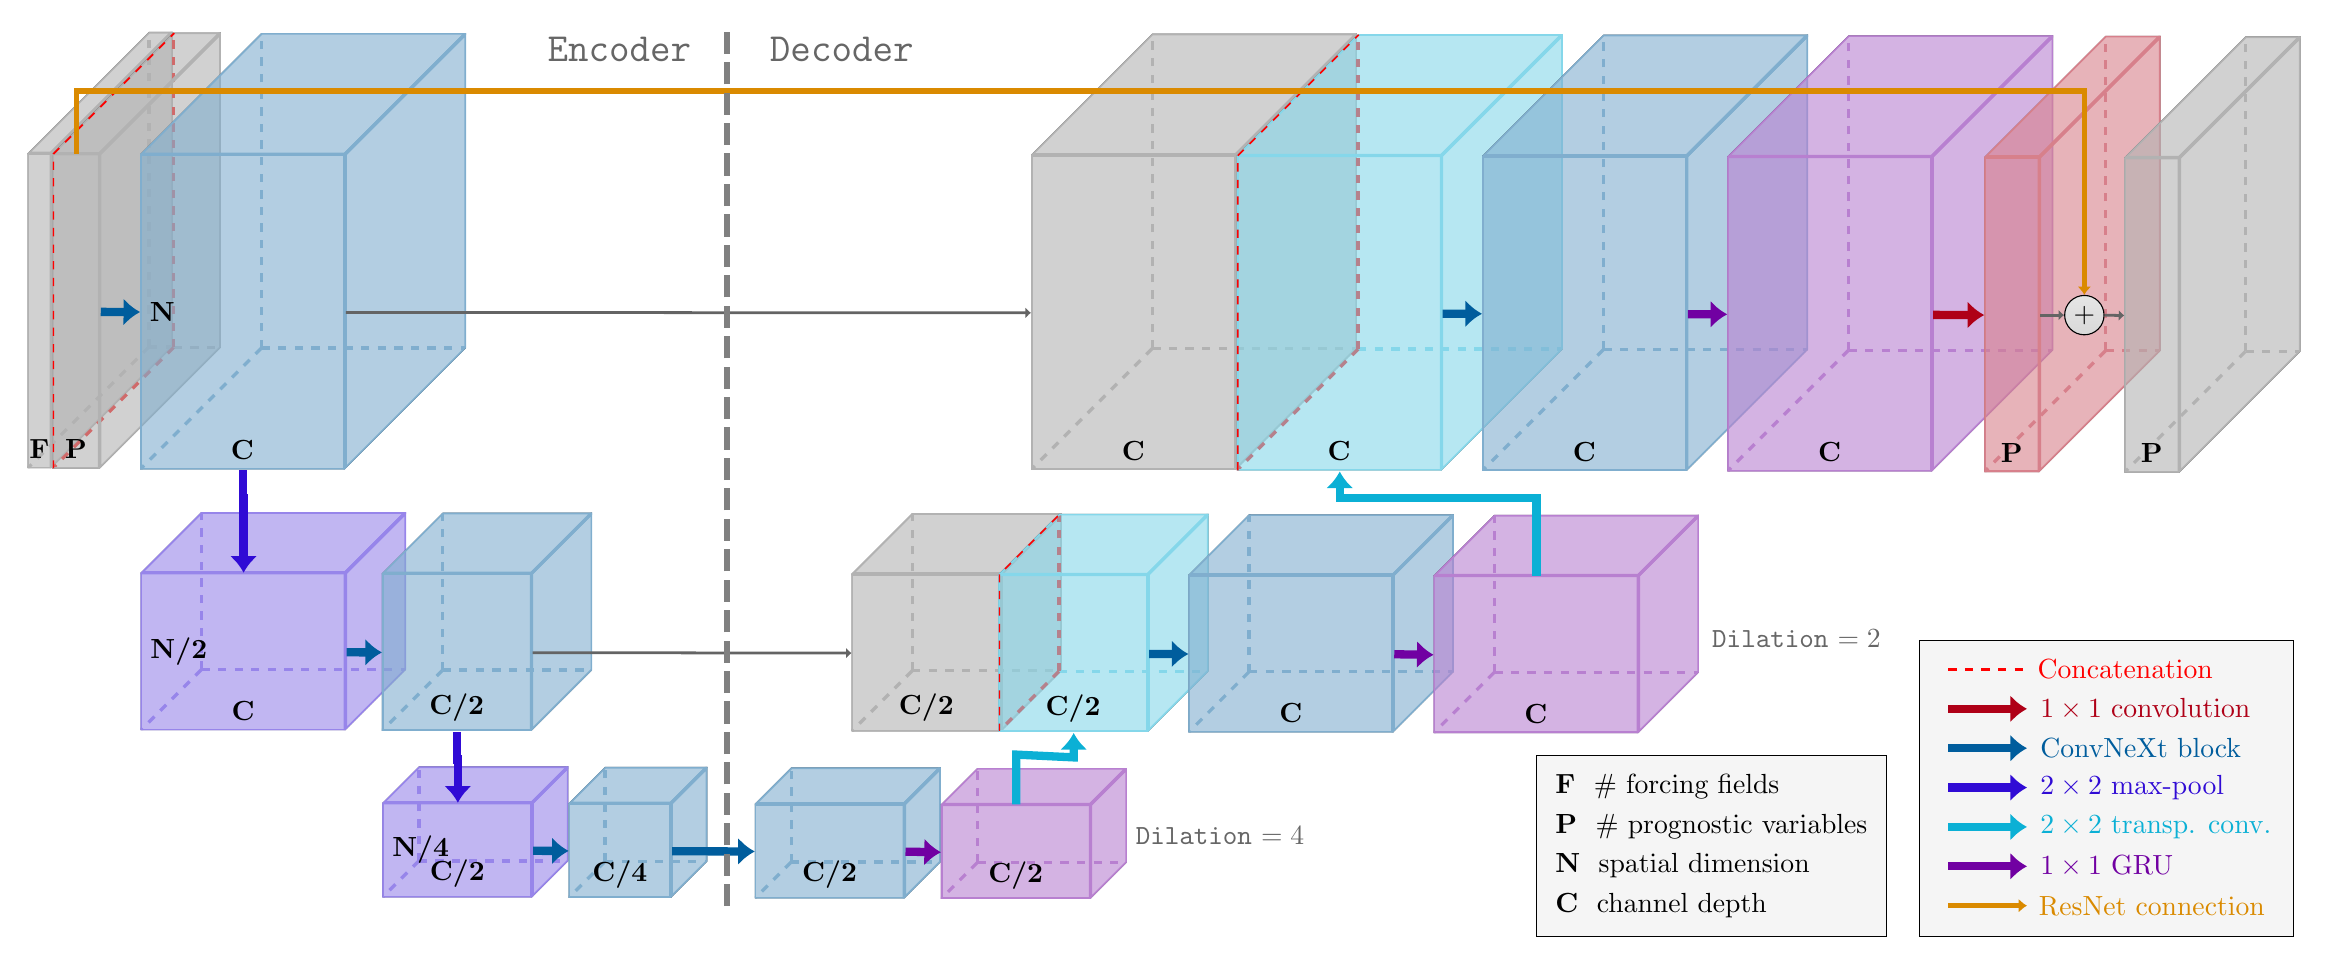
\begin{tikzpicture}
	
	%
	% First layer down
	
	% Maps
	\pic {annotated cuboid={width=0.3, height=4, depth=4, units=, label=forcing, lwidth=F, lheight=}};
	\pic [right=0.3cm of forcing] {annotated cuboid={width=0.6, height=4, depth=4, units=, label=prognostic, lwidth=P, lheight=, cat=1}};
	\pic [right=1.8cm of prognostic] {annotated cuboid={width=2.6, height=4, depth=4, units=, label=e1-1, lwidth=C, lheight=N, ccolor=white!50!convblockcolor}};
	
	% Arrows
	\draw[convblock] (prognostic) -- (e1-1);
	
	%
	% Second layer down
	
	% Maps
	\pic [below=2.3cm of e1-1] {annotated cuboid={width=2.6, height=2, depth=2, units=, label=e2-1, lwidth=C, lheight=N/2, ccolor=white!50!downscalecolor}};
	\pic [right=1.4cm of e2-1] {annotated cuboid={width=1.9, height=2, depth=2, units=, label=e2-2, lwidth=C/2, lheight=, ccolor=white!50!convblockcolor}};
	
	% Arrows
	\draw[downscale] (e1-1.south) --++ (0, -10pt) -- ([yshift=-10pt]e1-1.south -| e2-1.north) -- (e2-1.north);
	\draw[convblock] (e2-1) -- (e2-2);
	
	%
	% Third layer down (synoptic layer)
	
	% Maps
	\pic [below=1.5cm of e2-2] {annotated cuboid={width=1.9, height=1.2, depth=1.2, units=, label=e3-1, lwidth=C/2, lheight=N/4, ccolor=white!50!downscalecolor}};
	\pic [right=1.1cm of e3-1] {annotated cuboid={width=1.3, height=1.2, depth=1.2, units=, label=e3-2, lwidth=C/4, lheight=, ccolor=white!50!convblockcolor}};
	\pic [right=2.0cm of e3-2] {annotated cuboid={width=1.9, height=1.2, depth=1.2, units=, label=e3-3, lwidth=C/2, lheight=, ccolor=white!50!convblockcolor}};
	\pic [right=1.4cm of e3-3] {annotated cuboid={width=1.9, height=1.2, depth=1.2, units=, label=e3-4, lwidth=C/2, lheight=, ccolor=white!50!reccolor}};
	
	% Arrows
	\draw[downscale] (e2-2.south) --++ (0, -10pt) -- ([yshift=-10pt]e2-2.south -| e3-1.north) -- (e3-1.north);
	\draw[convblock] (e3-1) -- (e3-2);
	\draw[convblock] (e3-2) -- (e3-3);
	%\draw[rec] (e3-3.east) to [out=-45, in=-135, looseness=0.8] (e3-3.west);
	\draw[rec] (e3-3.east) -- (e3-4.west);
	
	% Dilation remark
	\node[yshift=0.2cm, right=2.8cm of e3-3, gray!80!black] {\texttt{Dilation} $= 4$};
	
	% Second layer up
	
	% Maps
	\pic [right=5.0cm of e2-2] {annotated cuboid={width=1.9, height=2, depth=2, units=, label=d2-1, lwidth=C/2, lheight=}};
	\pic [right=0.9cm of d2-1] {annotated cuboid={width=1.9, height=2, depth=2, units=, label=d2-2, lwidth=C/2, lheight=, ccolor=white!50!upscalecolor, cat=1}};
	\pic [right=1.8 of d2-2] {annotated cuboid={width=2.6, height=2, depth=2, units=, label=d2-3, lwidth=C, lheight=, ccolor=white!50!convblockcolor}};
	\pic [right=1.8 of d2-3] {annotated cuboid={width=2.6, height=2, depth=2, units=, label=d2-4, lwidth=C, lheight=, ccolor=white!50!reccolor}};
		
	% Arrows
	\draw[forward] (e2-2) -- (d2-1);
	\draw[upscale] (e3-4.north) --++ (0, 18pt) -- ([yshift=17pt]e3-4.north -| d2-2.south) -- (d2-2.south);
	\draw[convblock] (d2-2) -- (d2-3);
	%\draw[rec] (d2-3.east) to [out=-45, in=-135, looseness=1] (d2-3.west);
	\draw[rec] (d2-3.east) -- (d2-4.west);
	
	% Dilation remark
	\node[yshift=0.2cm, right=0.8cm of d2-4, gray!80!black] {\texttt{Dilation} $= 2$};
	
	%
	% First layer up
	
	\pic [right=10cm of e1-1] {annotated cuboid={width=2.6, height=4, depth=4, units=, label=d1-1, lwidth=C, lheight=}};
	\pic [right=1.3cm of d1-1] {annotated cuboid={width=2.6, height=4, depth=4, units=, label=d1-2, lwidth=C, lheight=, ccolor=white!50!upscalecolor, cat=1}};
	\pic [right=1.8 of d1-2] {annotated cuboid={width=2.6, height=4, depth=4, units=, label=d1-3, lwidth=C, lheight=, ccolor=white!50!convblockcolor}};
	\pic [right=1.8 of d1-3] {annotated cuboid={width=2.6, height=4, depth=4, units=, label=d1-4, lwidth=C, lheight=, ccolor=white!50!reccolor}};
	\pic [right=1.0 of d1-4] {annotated cuboid={width=0.7, height=4, depth=4, units=, label=d1-5, lwidth=P, lheight=, ccolor=white!50!convcolor}};
	\node[operator, right=0.3 of d1-5] (plus1) {$+$};
	\pic [right=0.6 of plus1] {annotated cuboid={width=0.7, height=4, depth=4, units=, label=d1-6, lwidth=P, lheight=}};

	% Arrows
	\draw[forward] (e1-1) -- (d1-1);
	\draw[upscale] (d2-4.north) --++ (0, 28pt) -- ([yshift=28pt]d2-4.north -| d1-2.south) -- (d1-2.south);
	\draw[convblock] (d1-2) -- (d1-3);
	\draw[rec] (d1-3) -- (d1-4);
	\draw[conv] (d1-4) -- (d1-5);
	\draw[forward] (d1-5) -- (plus1);
	\draw[skip] (prognostic.north) --++ (0, 0.8cm) -- ([yshift=0.8cm]prognostic.north -| plus1.north) -- (plus1.north);
	\draw[forward] (plus1) -- (d1-6);
	
	% Encoder/Decoder split
	%\tikzstyle{finndashed} = [dash pattern=on 2pt off 1.5pt]
	\draw[dash pattern=on 8pt off 3pt, line width=2pt, white!50!black] ([xshift=0.7cm, yshift=-0.7cm]e3-2.east) --++ (0, 11.1cm);
	\node[above=of e3-2, xshift=1.4cm, yshift=8.3cm] {\color{gray!80!black}\Large\texttt{\textbf{Encoder\hspace{1cm}Decoder}}};
	
	%
	% Legend
	\draw[cat] ([yshift=-2.5cm, xshift=1.5cm]d1-4.south) --++ (1, 0) node[right] (catlabel) {Concatenation};
	\draw[conv] ([yshift=-3.0cm, xshift=1.5cm]d1-4.south) --++ (1, 0) node[right] (convlabel) {$1\times1$ convolution};
	\draw[convblock] ([yshift=-3.5cm, xshift=1.5cm]d1-4.south) --++ (1, 0) node[right] (convblocklabel) {ConvNeXt block};
	\draw[downscale] ([yshift=-4.0cm, xshift=1.5cm]d1-4.south) --++ (1, 0) node[right] (downscalelabel) {$2\times2$ max-pool};
	\draw[upscale]([yshift=-4.5cm, xshift=1.5cm]d1-4.south) --++ (1, 0) node[right] (upscalelabel) {$2\times2$ transp. conv.};
	\draw[rec] ([yshift=-5.0cm, xshift=1.5cm]d1-4.south) --++ (1, 0) node[right] (reclabel) {$1\times1$ GRU};
	\draw[skip] ([yshift=-5.5cm, xshift=1.5cm]d1-4.south) --++ (1, 0) node[right] (skiplabel) {ResNet connection};
	\node[left=of catlabel] (legenddummy) {};
	\begin{pgfonlayer}{background}
		\node [draw, fill=gray!8!white, fit=(legenddummy) (catlabel) (convlabel) (convblocklabel) (downscalelabel) (upscalelabel) (reclabel) (skiplabel)] {};
	\end{pgfonlayer}
	
	\node[right] at ([yshift=-4.0cm, xshift=-0.5cm]d1-3.south) (flabel) {\textbf{F}\ \ \# forcing fields};
	\node[right] at ([yshift=-4.5cm, xshift=-0.5cm]d1-3.south) (plabel) {\textbf{P}\ \ \# prognostic variables};
	\node[right] at ([yshift=-5.0cm, xshift=-0.5cm]d1-3.south) (nlabel) {\textbf{N}\ \ spatial dimension};
	\node[right] at ([yshift=-5.5cm, xshift=-0.5cm]d1-3.south) (clabel) {\textbf{C}\ \ channel depth};
	\begin{pgfonlayer}{background}
		\node [draw, fill=gray!8!white, fit=(flabel) (plabel) (nlabel) (clabel)] {};
	\end{pgfonlayer}
		
	\end{tikzpicture}
\end{document}